\section{Introduction}

The estimation based on discrete time observations is in general difficult. The main obstacle is the fact that SDEs do not explicitly specify the conditional dynamics associated with the sampling process. The general framework is given by the following one-dimensional (It\^{o}) SDE:
\begin{equation}\label{eq01}
  dX_{t}= f(t,X_{t},\underline{\theta}) dt + g(t,X_{t},\underline{\theta}) dW_{t}, \quad \quad t \geq 0 \, , X_{0} = x_{0},
\end{equation}
where ${W}_{t}$ is a standard Wiener process, $f:\Theta \times [0,T] \times \mathbb{R} \rightarrow \mathbb{R}$, called the drift coefficient, and $g:\Xi \times [ 0 , T ] \times \mathbb{R} \rightarrow \mathbb{R}^{+}$, called the diffusion coefficient, are known functions except the unknown parameters $\underline{\theta}$, $\Theta \subset \mathbb{R}$, $\Xi \subset \mathbb{R}$ and $\E(X_{0}^{2}) < \infty$. Parameters $\underline{\theta}$ in \eqref{eq01} are crucial for the characterization of dynamic phenomena being considered, naturally, researchers are interested in obtaining better estimates of the parameters using the observation data. There a rich literature and many books with applications in different fields and computer vision, e.g., \cite{Prakasa1999,Sorensen2000,Kutoyants2004,Stefano2008,Stefano2011}. In practical situations the available data are discrete time series (in \R~class \code{'ts'}) data sampled over some time interval. Thus, the parameter estimation for discretely observed SDE is non-trivial and during the past decades it has generated a great deal of research effort, and has attracted the attention of lot of
researchers. The following list is an attempt to summarise some contributions, despite the great number. However, it is certainly not a complete reference of the subject of the techniques to estimate in SDE's (e.g. \cite{DacunhaandFlorens1986,Dohnal1987,Florens1989,Genon1990,Ozaki1992,Yoshida1992,Pedersen1995,Kloedenetall1996,Kessler1997,GallantandLong1997,ShojiandOzaki1997,ShojiandOzaki1998,HurnandLindsay1999,Florens1999,AitSahalia1999,AitSahalia2002,Nicolau2002,Nicolau2004,Sorensen2000,Sorensen2002,Sorensen2004,Hurnetall2003,AlcockandBurrage2004,OgiharaandYoshida2011,UchidaandYoshida2012,BrousteandStefano2013},$\dots$)
to the best of our knowledge.

There already exist a number of packages that can perform for estimation of SDE's with different methods in~\cite{R}; see \CRANpkg{sde}~\citep{Stefano2009} it is the accompanying package to the book of~\citep{Stefano2008}. The \CRANpkg{yuima} project package~\citep{Stefano2014} for simulation and inference for (multidimensional) SDE's; and \CRANpkg{PSM} package~\citep{StigandSoren2013} for estimation of linear and non-linear mixed-effects models using SDE's, are freely available on CRAN. The package \CRANpkg{Sim.DiffProc}~\citep{Sim.DiffProc} contains specific function \code{fitsde} for pseudo-maximum likelihood (also denoted quasi-maximum likelihood) estimators for one-dimensional SDE's, we implement four approximation scheme: \textbf{Euler}\footnote{The implementation of this method in \R~is very easy see~\citet[p. 122]{Stefano2008}.} \citep{Florens1989,Yoshida1992}, \textbf{Ozaki}\footnote[2]{The functions \code{dcOzaki}, \code{dcShoji} and \code{dcKessler} are available on \pkg{sde} package~\citet{Stefano2009}, for approximated conditional law of a diffusion process.} \citep{Ozaki1992}, \textbf{Shoji-Ozaki}\footnotemark[2] \citep{ShojiandOzaki1998} and \textbf{Kessler}\footnotemark[2] method \citep{Kessler1997}. These approximation schemes do not approximate the transition density of \eqref{eq01} directly but the path of the process $X_t$ in such a way that the discretized version of the process has a likelihood that is usable.

\section{Pseudo-likelihood methods}

To simplify equation \eqref{eq01}, suppose that the infinitesimal coefficients do not depend on $t$, i.e. consider:
\begin{equation}\label{eq02}
  dX_{t}= f(X_{t},\underline{\theta}) dt + g(X_{t},\underline{\theta}) dW_{t}, \quad \quad t \geq 0 \, , X_{0} = x_{0},
\end{equation}
$X_t$ is a time-homogeneous process. In this case the transition density (which we always assume to exist) depends only on $\Delta t$, $x$ and $y$. Hence, we can write it in the form $p(\Delta t,x,y)$ (or $p(t_{i-1},x,t_{i},y)$). If $\Delta t$ is constant and some regularity conditions it is known that $p(t-s,x,y)$ satisfies the equation of Fokker-Planck backward, it focuses on the variable $x$ starting,
\begin{equation}\label{eq03}
  \frac{\partial p}{\partial s} = f(x) \frac{\partial p}{\partial x} + \frac{1}{2}g^{2}(x)\frac{\partial^{2}p }{\partial x^{2}} ,
\end{equation}
Only in simple cases can we solve these Partial differential equation (PDEs). Since the transition densities are generally unknown we cannot in principle obtain the $\MLE$. Nevertheless, we will see some methods that can estimate these densities. With initial condition $X_0$ and $\theta$ the $\mathrm{p}$-dimensional parameter of interest, by Markov property of diffusion processes, the likelihood has this form:
\begin{equation}\label{eq04}
  L_{n}(\theta)=\prod_{i=1}^{n} \log p_{\theta}(\Delta t, X_{i-1},X_{i}) p_{\theta}(X_{0}),
\end{equation}
and the log-likelihood is:
\begin{equation}\label{eq05}
  l_{n}(\theta)=\log L_{n}(\theta)=\sum_{i=1}^{n} \log p_{\theta}(\Delta t, X_{i-1},X_{i}) + \log (p_{\theta}(X_{0})),
\end{equation}
\eqref{eq05} be the log-likelihood function associated with the \eqref{eq02}. If some conditional moments of $X_t$ are known but not the true transition density $p$, it is possible to estimate $\theta$ from a density $h$ that although not belonging to the family of the true conditional density, is compatible in terms of moments with $p$. The $h$ density is denoted as the pseudo true density. The pseudo maximum likelihood ($\PMLE$) is defined as the solution of the following optimization problem:
\begin{equation}\label{eq06}
\hat{\theta}_{n}=\argmax {\theta \in \Theta} h_{n}(\theta|X_{1},X_{2},\dots,X_{n}),
\end{equation}
with:
\begin{equation}\label{eq07}
  h_{n}(\theta|X_{1},X_{2},\dots,X_{n})=\sum_{i=1}^{n} \log h_{\theta}(\Delta t, X_{i-1},X_{i}) + \log (h_{\theta}(X_{0})),
\end{equation}
Under some conditions this techniques apply to high frequency data i.e., $\Delta t \rightarrow 0$ and $n \Delta t \rightarrow +\infty$.

The \pkg{Sim.DiffProc} package implements $\PMLE$ via the \code{fitsde} function. The interface and the output of the \code{fitsde} function are made as similar as possible to those of the standard \code{mle} function in the \pkg{stats4} package of the basic \R~system. The main arguments to \code{fitsde} consist of a \code{data} of type a univariate time series (\code{ts} object) and initial values (\code{start}) for the optimizer. The \code{drift} and \code{diffusion} indicate drift and diffusion coefficient of the model \eqref{eq01}, is an \code{expression} of two variables \code{t}, \code{x} and \code{theta} names of the parameters, and must be nominated by a vector of \code{theta = (theta[1], theta[2],..., theta[p])} for reasons of symbolic derived in approximation methods. The \code{start} argument must be specified as a named list, where the names of the elements of the list correspond to the names of the parameters as they appear in the \code{drift} and \code{diffusion} coefficient. The \code{pmle} argument must be a \code{character} string specifying the method to use, can be either: \code{"euler"}, \code{"ozaki"}, \code{"shoji"} and \code{"kessler"}. We can select the optimization method by the argument \code{optim.method} (\code{"L-BFGS-B"} is used by default), and further arguments to pass to \code{optim} function. The following we explain how to use this function to estimate a model \eqref{eq01} with different approximation methods, as well as other functions of type \code{'S3'} are linking to a class \code{'fitsde'}.

\subsection{Euler method}

Consider a process solution of the general stochastic differential equation \eqref{eq02}, the Euler scheme produces the discretization ($\Delta t \rightarrow 0$):
\begin{equation*}
X_{t+\Delta t} - X_{t} = f(X_{t},\theta) \Delta t+ g(X_{t},\theta) (W_{t+\Delta t} -W_{t}),
\end{equation*}
the increments $X_{t+\Delta t} - X_{t}$ are then independent Gaussian random variables with mean: $\E_{x} = f(X_{t},\theta)\Delta t$, and variance: $\V_{x} = g^{2}(X_{t},\theta) \Delta t$. Therefore the transition
density of the process can be written as:
\begin{equation*}
  p_{\theta}(t,y|x)=\frac{1}{\sqrt{2\pi t g^{2}(x,\theta)}} \exp\left(-\frac{\left(y-x-f(x,\theta)t\right)^2}{2tg^{2}(x,\theta)}\right)
\end{equation*}
then the log-likelihood is:
\begin{equation}\label{eq08}
  h_{n}(\theta|X_{1},X_{2},\dots,X_{n})=-\frac{1}{2}\left(\sum_{i=1}^{n} \frac{(X_{i}-X_{i-1}-f(X_{i-1},\theta)\Delta)^2}{\sigma^2 \Delta t} + n \log(2\pi \sigma^2 \Delta t)\right)
\end{equation}
the equation above is also called the locally Gaussian approximation. \cite{Florens1989} and \cite{Yoshida1992} showed that a consistent estimator of $\sigma^2$ is:
$$
\hat{\sigma}^2 = \frac{1}{n \Delta t} \sum_{i=1}^{n} (X_{i}-X_{i-1})^2
$$
As an example, we consider the Chan-Karolyi-Longstaff-Sanders (CKLS) model:
\begin{equation}\label{eq09}
  dX_{t} = (\theta_{1}+\theta_{2} X_{t}) dt + \theta_{3} X_{t}^{\theta_{4}} dW_{t},\qquad X_{0}=2
\end{equation}
with $\theta_{1}=1$, $\theta_{2}=2$, $\theta_{3}=0.5$ and $\theta_{4}=0.3$. Before calling \code{fitsde}, we generate sampled data $X_{t_{i}}$, with $\Delta t =10^{-3}$, as following:
\begin{Schunk}
\begin{Sinput}
> f <- expression( (1+2*x) )
> g <- expression( 0.5*x^0.3 )
> sim    <- snssde1d(drift=f,diffusion=g,x0=2,M=1,N=1000,Dt=0.001)
> mydata <- sim$X
\end{Sinput}
\end{Schunk}
we set the initial values for the optimizer as $\theta_{1}=\theta_{2}=\theta_{3}=\theta_{4}=1$, and we specify the coefficients drift and diffusion as expressions.
you can use the \code{upper} and \code{lower} limits of the search region used by the optimizer (here using the default method \code{"L-BFGS-B"}), and specifying the method to use with \code{pmle="euler"}.
We can now use the function \code{fitsde} to estimate the parameters of \eqref{eq09} as follows:
\begin{Schunk}
\begin{Sinput}
> fx <- expression( theta[1]+theta[2]*x ) ## drift coefficient of model (9)
> gx <- expression( theta[3]*x^theta[4] ) ## diffusion coefficient of model (9)
> fitmod <- fitsde(data=mydata,drift=fx,diffusion=gx,start = list(theta1=1,
+                  theta2=1,theta3=1,theta4=1),pmle="euler")
\end{Sinput}
\end{Schunk}
The estimated coefficients are extracted from the output object \code{fitmod} as follows:
\begin{Schunk}
\begin{Sinput}
> coef(fitmod)
\end{Sinput}
\begin{Soutput}
   theta1    theta2    theta3    theta4
1.1201172 2.1384034 0.5288006 0.2701521
\end{Soutput}
\end{Schunk}
we can use the \code{summary} function to produce result summaries of output object \code{fitmod}:
\begin{Schunk}
\begin{Sinput}
> summary(fitmod)
\end{Sinput}
\begin{Soutput}
Pseudo maximum likelihood estimation

Method:  Euler
Call:
fitsde(data = mydata, drift = fx, diffusion = gx, start = list(theta1 = 1,
    theta2 = 1, theta3 = 1, theta4 = 1), pmle = "euler")

Coefficients:
        Estimate Std. Error
theta1 1.1201172 1.57355762
theta2 2.1384034 0.19229249
theta3 0.5288006 0.03752510
theta4 0.2701521 0.03479513

-2 log L: -4298.304
\end{Soutput}
\end{Schunk}
The functions of type \code{S3} method (as similar of the standard \code{mle} function in the \pkg{stats4} package of the basic \R~system) for the class \code{'fitsde'} are the following:
\begin{itemize}
  \item [$\circ$] \code{coef}: which extracts model coefficients from objects returned by \code{'fitsde'}.
  \item [$\circ$] \code{vcov}: returns the variance-covariance matrix of the parameters of a fitted model objects.
  \item [$\circ$] \code{logLik}: extract log-likelihood.
  \item [$\circ$] \code{AIC}: calculating Akaike's Information Criterion for fitted model objects.
  \item [$\circ$] \code{BIC}: calculating Schwarz's Bayesian Criterion for fitted model objects.
  \item [$\circ$] \code{confint}: computes confidence intervals for one or more parameters in a fitted model objects.
\end{itemize}
\begin{Schunk}
\begin{Sinput}
> vcov(fitmod)
\end{Sinput}
\begin{Soutput}
             theta1        theta2        theta3        theta4
theta1  2.476083599 -0.2524732417 -0.0038764366  0.0038346123
theta2 -0.252473242  0.0369764031  0.0004688301 -0.0004628819
theta3 -0.003876437  0.0004688301  0.0014081329 -0.0012391759
theta4  0.003834612 -0.0004628819 -0.0012391759  0.0012107014
\end{Soutput}
\begin{Sinput}
> AIC(fitmod)
\end{Sinput}
\begin{Soutput}
[1] -4290.304
\end{Soutput}
\begin{Sinput}
> confint(fitmod, level=0.95)
\end{Sinput}
\begin{Soutput}
            2.5 %    97.5 %
theta1 -1.9639990 4.2042335
theta2  1.7615170 2.5152898
theta3  0.4552527 0.6023484
theta4  0.2019549 0.3383494
\end{Soutput}
\end{Schunk}

\subsection{Ozaki method}

The second approach we present is the Ozaki method (\citet{Ozaki1992,ShojiandOzaki1997}), and it works for homogeneous stochastic differential equations. Consider the stochastic differential
equation:
\begin{equation}\label{eq10}
  dX_{t}= f(X_{t},\underline{\theta}) dt + \sigma dW_{t}, \quad \quad t \geq 0 \, , X_{0} = x_{0},
\end{equation}
where $\sigma$ is supposed to be constant. We just recall that the transition density for the Ozaki method is Gaussian, we have that: $X_{t+\Delta t}|X_{t} = x \sim \mathcal{N}(\E_{x},\V_{x})$, where:
\begin{align}\label{eq11}
  \E_{x} &= x + \frac{f(x)}{\partial_{x} f(x)} \left( e^{\partial_{x} f(x) \Delta t} - 1 \right), \\
  \V_{x} &= \sigma^{2} \frac{e^{2K_{x} \Delta t} -1}{2K_{x}},
\end{align}
with:
\begin{equation*}
  K_{x} = \frac{1}{\Delta t} \log \left(1+\frac{f(x)}{x\partial_{x}f(x)}\left(e^{\partial_{x}f(x) \Delta t}-1\right) \right)
\end{equation*}
It is always possible to transform equation \eqref{eq02} with a constant diffusion coefficient using the Lamperti transform (see \cite{ShojiandOzaki1998,Florens1999,AitSahalia2002} and \citet[p. 40]{Stefano2008}).

Now we consider the Vasicek model, with $f(x,\theta) = \theta_{1} (\theta_{2}- x)$ and constant
volatility $g(x,\theta) = \theta_{3}$,
\begin{equation}\label{eq12}
  dX_{t} = \theta_{1} (\theta_{2}- X_{t}) dt + \theta_{3} dW_{t},\qquad X_{0}=5
\end{equation}
with $\theta_{1}=3$, $\theta_{2}=2$ and $\theta_{3}=0.5$, we generate sampled data $X_{t_{i}}$, with $\Delta t =10^{-2}$, as following:
\begin{Schunk}
\begin{Sinput}
> f <- expression( 3*(2-x) )
> g <- expression( 0.5 )
> sim <- snssde1d(drift=f,diffusion=g,x0=5,Dt=0.01)
> HWV <- sim$X
\end{Sinput}
\end{Schunk}
we set the initial values for the optimizer as $\theta_{1}=\theta_{2}=\theta_{3}=1$, and we specify the coefficients drift and diffusion as expressions.
Specifying the method to use with \code{pmle="ozaki"}, which can easily be implemented in \R~as follows:
\begin{Schunk}
\begin{Sinput}
> fx <- expression( theta[1]*(theta[2]- x) ) ## drift coefficient of model (13)
> gx <- expression( theta[3] )           ## diffusion coefficient of model (13)
> fitmod <- fitsde(data=HWV,drift=fx,diffusion=gx,start = list(theta1=1,theta2=1,
+                  theta3=1),pmle="ozaki")
> summary(fitmod)
\end{Sinput}
\begin{Soutput}
Pseudo maximum likelihood estimation

Method:  Ozaki
Call:
fitsde(data = HWV, drift = fx, diffusion = gx, start = list(theta1 = 1,
    theta2 = 1, theta3 = 1), pmle = "ozaki")

        Estimate Std. Error
theta1 3.0844858 0.56115144
theta2 1.9897618 0.22305649
theta3 0.4675424 0.03306254

-2 log L: -329.5772
\end{Soutput}
\end{Schunk}
If you want to have confidence intervals $\theta_{1}$ and $\theta_{2}$ parameters only, using the command \code{confint} as following:
\begin{Schunk}
\begin{Sinput}
> confint(fitmod,parm=c("theta1","theta2"),level=0.95)
\end{Sinput}
\begin{Soutput}
          2.5 %   97.5 %
theta1 1.984649 4.184322
theta2 1.552579 2.426944
\end{Soutput}
\end{Schunk}

\subsection{Shoji-Ozaki method}
An extension of the method to Ozaki the more general case where the drift is allowed to depend on the time variable $t$, and also the diffusion coefficient can be varied is the method \citet{ShojiandOzaki1998}. Consider the stochastic differential
equation:
\begin{equation}\label{eq13}
  dX_{t}= f(t,X_{t},\underline{\theta}) dt + g(X_{t},\underline{\theta}) dW_{t}, \quad \quad t \geq 0 \, , X_{0} = x_{0},
\end{equation}
the transition density for the Shoji-Ozaki method is Gaussian, we have that: $X_{t+\Delta t}|X_{t} = x \sim \mathcal{N}\left(\mathrm{A}_{(t,x)}x,\mathrm{B}^{2}_{(t,x)}\right)$, where:
\begin{align}\label{eq14}
  \mathrm{A}_{(t,x)} &= 1+ \frac{f(t,x)}{x\mathrm{L}_{t}} \left(e^{\mathrm{L}_{t}\Delta t }-1\right)+\frac{\mathrm{M}_{t}}{x\mathrm{L}^{2}_{t}} \left(e^{\mathrm{L}_{t} \Delta t}-1-\mathrm{L}_{t}\Delta t\right), \\
  \mathrm{B}_{(t,x)} &= g(x) \sqrt{\frac{e^{2\mathrm{L}_{t} \Delta t}-1}{2\mathrm{L}_{t}}},
\end{align}
with:
\begin{equation*}
  \mathrm{L}_{t} = \partial_{x} f(t,x) \quad\text{and}\quad  \mathrm{M}_{t} = \frac{g^{2}(x)}{2} \partial_{xx} f(t,x)+ \partial_{t} f(t,x).
\end{equation*}
for more details, can be found in the original works \citet{ShojiandOzaki1997,ShojiandOzaki1998}. As an example, we consider the following model:
\begin{equation}\label{eq15}
  dX_{t} = a(t)X_{t} dt + \theta_{2}X_{t} dW_{t},\qquad X_{0}=10
\end{equation}
with: $a(t) = \theta_{1}t$, and we generate sampled data $X_{t_{i}}$, with $\theta_{1}=-2$, $\theta_{2}=0.2$ and time step $\Delta t =10^{-3}$, as following:
\begin{Schunk}
\begin{Sinput}
> f <- expression(-2*x*t)
> g <- expression(0.2*x)
> sim <- snssde1d(drift=f,diffusion=g,N=1000,Dt=0.001,x0=10)
> mydata <- sim$X
\end{Sinput}
\end{Schunk}
we set the initial values for the optimizer as $\theta_{1}=\theta_{2}=1$, and we specify the method to use with \code{pmle="shoji"},
\begin{Schunk}
\begin{Sinput}
> fx <- expression( theta[1]*x*t ) ## drift coefficient of model (17)
> gx <- expression( theta[2]*x )   ## diffusion coefficient of model (17)
> fitmod <- fitsde(data=mydata,drift=fx,diffusion=gx,start = list(theta1=1,
+                  theta2=1),pmle="shoji")
> summary(fitmod)
\end{Sinput}
\begin{Soutput}
Pseudo maximum likelihood estimation

Method:  Shoji
Call:
fitsde(data = mydata, drift = fx, diffusion = gx, start = list(theta1 = 1,
    theta2 = 1), pmle = "shoji")

Coefficients:
         Estimate  Std. Error
theta1 -1.9994423 0.347451420
theta2  0.2004914 0.004485035

-2 log L: -3033.682
\end{Soutput}
\begin{Sinput}
> vcov(fitmod)
\end{Sinput}
\begin{Soutput}
              theta1        theta2
theta1  1.207225e-01 -6.058961e-06
theta2 -6.058961e-06  2.011554e-05
\end{Soutput}
\begin{Sinput}
> logLik(fitmod)
\end{Sinput}
\begin{Soutput}
[1] 1516.841
\end{Soutput}
\begin{Sinput}
> confint(fitmod,level=0.9)
\end{Sinput}
\begin{Soutput}
              5 %      95 %
theta1 -2.5709490 -1.4279356
theta2  0.1931142  0.2078686
\end{Soutput}
\end{Schunk}

\subsection{Kessler method}

\citet{Kessler1997} proposed to use a higher-order It\^{o}-Taylor expansion to approximate the mean and variance in a conditional Gaussian density. Consider the stochastic differential equation \eqref{eq01}, the transition density by Kessler method is: $X_{t+\Delta t}|X_{t} = x \sim \mathcal{N}\left(\E_{x},\V_{x}\right)$, where:
\begin{align}\label{eq16}
  \E_{x} &= x + f(t,x) \Delta t+\left(f(t,x)\partial_{x}f(t,x) + \frac{1}{2} g^{2}(t,x) \partial_{xx}g(t,x)\right)\frac{(\Delta t)^2}{2}, \\
  \V_{x} &= x^2 +(2f(t,x)x+g^{2}(t,x)) \Delta t +\bigg(2f(t,x)\left(\partial_{x}f(t,x)x+f(t,x)+g(t,x)\partial_{x}g(t,x)\right) \nonumber\\
         &\quad+g^{2}(t,x)\left(\partial_{xx}f(t,x)x+2\partial_{x}f(t,x)+\partial_{x}g^{2}(t,x)+g(t,x)\partial_{xx}g(t,x)\right)\bigg)\frac{(\Delta t)^2}{2}-\E^{2}_{x}.
\end{align}
In the framework consider by this approximation, see \citet{Kessler1997} for the result  for the maximum likelihood estimator.

We consider the following Hull-White (extended Vasicek) model:
\begin{equation}\label{eq17}
  dX_{t} = a(t)(b(t)-X_{t}) dt + \sigma(t) dW_{t},\qquad X_{0}=2
\end{equation}
with: $a(t) = \theta_{1}t$ and $b(t)=\theta_{2}\sqrt{t}$, the volatility depends on time: $\sigma(t)=\theta_{3}t$. We generate sampled data of \eqref{eq17}, with $\theta_{1}=3$, $\theta_{2}=1$ and $\theta_{3}=0.3$, time step $\Delta t =10^{-3}$, as following:
\begin{Schunk}
\begin{Sinput}
> f <- expression(3*t*(sqrt(t)-x))
> g <- expression(0.3*t)
> sim <- snssde1d(drift=f,diffusion=g,M=1,N=1000,x0=2,Dt=0.001)
> mydata <- sim$X
\end{Sinput}
\end{Schunk}
we set the initial values for the optimizer as $\theta_{1}=\theta_{2}=\theta_{3}=1$, and we specify the method to use with \code{pmle="kessler"},
\begin{Schunk}
\begin{Sinput}
> ## drift coefficient of model (20)
> fx <- expression( theta[1]*t* ( theta[2]*sqrt(t) - x ) )
> ## diffusion coefficient of model (20)
> gx <- expression( theta[3]*t )
> fitmod <- fitsde(data=mydata,drift=fx,diffusion=gx,start = list(theta1=1,
+                  theta2=1,theta3=1),pmle="kessler")
> summary(fitmod)
\end{Sinput}
\begin{Soutput}
Pseudo maximum likelihood estimation

Method:  Kessler
Call:
fitsde(data = mydata, drift = fx, diffusion = gx, start = list(theta1 = 1,
    theta2 = 1, theta3 = 1), pmle = "kessler")

Coefficients:
        Estimate  Std. Error
theta1 3.1334952 0.333744885
theta2 1.1253709 0.158830540
theta3 0.2957026 0.006615639

-2 log L: -8492.931
\end{Soutput}
\end{Schunk}
\section{The \texttt{fitsde()} in practice}

\subsection{Estimation of attractive model}

We propose the following dispersion models family \citep{Boukhetala1996}:
\begin{equation}\label{eq18}
    dR_t = \left( \frac{0.5 \theta^{2}_{3} R_t^{ \theta_{2} - 1} - \theta_{1}}{R_t^{\theta_{2}}} \right) dt + \theta_{3} dW_{t},
\end{equation}
where: $2 \theta_{1}> \theta^{2}_{3}$ condition to ensure attractiveness; we generate sampled data of this model, with
$\theta_{1}=5$, $\theta_{2}=1$ and $\theta_{3}=0.2$, $\Delta t =10^{-3}$, as following:
\begin{Schunk}
\begin{Sinput}
> theta1 = 5; theta2 = 1; theta3 = 0.2
> f <- expression( ((0.5*theta3^2 *x^(theta2-1) - theta1)/ x^theta2) )
> g <- expression( theta3 )
> sim <- snssde1d(drift=f,diffusion=g,M=1,N=1000,x0=3,Dt=0.001)
> mydata <- sim$X
\end{Sinput}
\end{Schunk}
we use \code{fitsde} function to estimate the parameters of model \eqref{eq18} as follows:
\begin{Schunk}
\begin{Sinput}
> fx <- expression( ((0.5*theta[3]^2 *x^(theta[2]-1) - theta[1])/ x^theta[2])  )
> gx <- expression(theta[3])
> fitmod <- fitsde(mydata,drift=fx,diffusion=gx, start = list(theta1=1,theta2=1,
+                 theta3=1),pmle="euler")
> coef(fitmod)
\end{Sinput}
\begin{Soutput}
   theta1    theta2    theta3
5.0176690 1.0077608 0.2040635
\end{Soutput}
\end{Schunk}
for to calculate the bias and confidence intervals of estimators it is easy, we can proceed as follows:
\begin{Schunk}
\begin{Sinput}
> true <- c(theta1,theta2,theta3)   ## True parameters
> bias <- true-coef(fitmod)
> bias
\end{Sinput}
\begin{Soutput}
      theta1       theta2       theta3
-0.017669042 -0.007760805 -0.004063473
\end{Soutput}
\begin{Sinput}
> confint(fitmod)
\end{Sinput}
\begin{Soutput}
           2.5 %    97.5 %
theta1 4.4894051 5.5459330
theta2 0.9594991 1.0560225
theta3 0.1951120 0.2130149
\end{Soutput}
\end{Schunk}
\subsection{Model selection via AIC}
The aim is to try to identify the underlying continuous model on the basis of discrete observations using AIC (Akaike Information Criterion) statistics.
\citet{UchidaandYoshida2005} develop the AIC statistics defined as:
\begin{equation}\label{eq19}
  \mathrm{AIC} = -2h_{n}\left(\hat{\theta}^{\mathrm{PML}}_{n}\right) + 2 \mathrm{dim}(\Theta),
\end{equation}
where $\hat{\theta}^{\mathrm{PML}}_{n}$ is the pseudo maximum likelihood estimator and $h_{n}$ the local Gaussian
approximation of the true log-likelihood. When comparing several models for a given data set, the models such that the AIC is lower is preferred.

Let the following models:
\begin{align*}
% \nonumber to remove numbering (before each equation)
  dX_{t} &= \theta_{1} X_{t} dt + \theta_{2} X_{t}^{\theta_{3}} dW_{t},             &\text{(true model)}\\
  dX_{t} &= (\theta_{1}+\theta_{2} X_{t}) dt + \theta_{3} X_{t}^{\theta_{4}} dW_{t},&\text{(competing model 1)}\\
  dX_{t} &= (\theta_{1}+\theta_{2} X_{t}) dt + \theta_{3} \sqrt{X_{t}} dW_{t},      &\text{(competing model 2)}\\
  dX_{t} &= \theta_{1} dt + \theta_{2} X_{t}^{\theta_{3}} dW_{t},                   &\text{(competing model 3)}
\end{align*}
We generate data from true model with parameters $\underline{\theta}=(2,0.3,0.5)$, initial value $X_{0}=2$ and $\Delta t =10^{-3}$, as following:
\begin{Schunk}
\begin{Sinput}
> f <- expression( 2*x )
> g <- expression( 0.3*x^0.5 )
> sim <- snssde1d(drift=f,diffusion=g,M=1,N=1000,x0=2,Dt=0.001)
> mydata <- sim$X
\end{Sinput}
\end{Schunk}
We test the performance of the AIC statistics for the four competing models, we can proceed as follows:
\begin{Schunk}
\begin{Sinput}
> ## True model
> fx <- expression( theta[1]*x )
> gx <- expression( theta[2]*x^theta[3] )
> truemod <- fitsde(data=mydata,drift=fx,diffusion=gx,start = list(theta1=1,
+                   theta2=1,theta3=1),pmle="euler")
> ## competing model 1
> fx1 <- expression( theta[1]+theta[2]*x )
> gx1 <- expression( theta[3]*x^theta[4] )
> mod1 <- fitsde(data=mydata,drift=fx1,diffusion=gx1,start = list(theta1=1,
+           theta2=1,theta3=1,theta4=1),pmle="euler")
> ## competing model 2
> fx2 <- expression( theta[1]+theta[2]*x )
> gx2 <- expression( theta[3]*sqrt(x) )
> mod2 <- fitsde(data=mydata,drift=fx2,diffusion=gx2,start = list(theta1=1,
+           theta2=1,theta3=1),pmle="euler")
> ## competing model 3
> fx3 <- expression( theta[1] )
> gx3 <- expression( theta[2]*x^theta[3] )
> mod3 <- fitsde(data=mydata,drift=fx3,diffusion=gx3,start = list(theta1=1,
+           theta2=1,theta3=1),pmle="euler")
> ## Computes AIC
> AIC <- c(AIC(truemod),AIC(mod1),AIC(mod2),AIC(mod3))
> Test <- data.frame(AIC,row.names = c("True mod","Comp mod1","Comp mod2",
+                    "Comp mod3"))
> Test
\end{Sinput}
\begin{Soutput}
                AIC
True mod  -4867.597
Comp mod1 -4865.617
Comp mod2 -4867.587
Comp mod3 -4810.597
\end{Soutput}
\begin{Sinput}
> Bestmod <- rownames(Test)[which.min(Test[,1])]
> Bestmod
\end{Sinput}
\begin{Soutput}
[1] "True mod"
\end{Soutput}
\end{Schunk}
the estimates under the different models,
\begin{Schunk}
\begin{Sinput}
> Theta1 <- c(coef(truemod)[[1]],coef(mod1)[[1]],coef(mod2)[[1]],coef(mod3)[[1]])
> Theta2 <- c(coef(truemod)[[2]],coef(mod1)[[2]],coef(mod2)[[2]],coef(mod3)[[2]])
> Theta3 <- c(coef(truemod)[[3]],coef(mod1)[[3]],coef(mod2)[[3]],coef(mod3)[[3]])
> Theta4 <- c("",coef(mod1)[[4]],"","")
> Parms  <- data.frame(Theta1,Theta2,Theta3,Theta4,row.names = c("True mod",
+                      "Comp mod1","Comp mod2","Comp mod3"))
> Parms
\end{Sinput}
\begin{Soutput}
              Theta1    Theta2    Theta3    Theta4
True mod   1.8978518 0.3007418 0.4928129        
Comp mod1 -0.1776481 1.9283156 0.3007623 0.4927636
Comp mod2 -0.1742726 1.9276524 0.2972557 
Comp mod3  8.2200670 0.2914395 0.5297354 
\end{Soutput}
\end{Schunk}

\subsection{Application to real data}
We make use of real data of the U.S. Interest Rates monthly form $06/1964$ to $12/1989$ (see Figure \ref{fig1}) available in package \pkg{Ecdat} \citep{Croissant2014}, and we estimate the parameters $\underline{\theta}=(\theta_{1},\theta_{2},\theta_{3},\theta_{4})$ of CKLS model \eqref{eq09}. These data have been analyzed by \citet{Stefano2014} with \pkg{yuima} package, here we confirm the results of the estimates by several approximation methods.
\begin{Schunk}
\begin{Sinput}
> data(Irates)
> rates <- Irates[, "r1"]
> X <- window(rates, start = 1964.471, end = 1989.333)
\end{Sinput}
\end{Schunk}
\begin{Schunk}
\begin{Sinput}
> plot(X)
\end{Sinput}
\end{Schunk}
\setkeys{Gin}{width=0.6\textwidth}
\begin{figure}[!ht]
\begin{center}
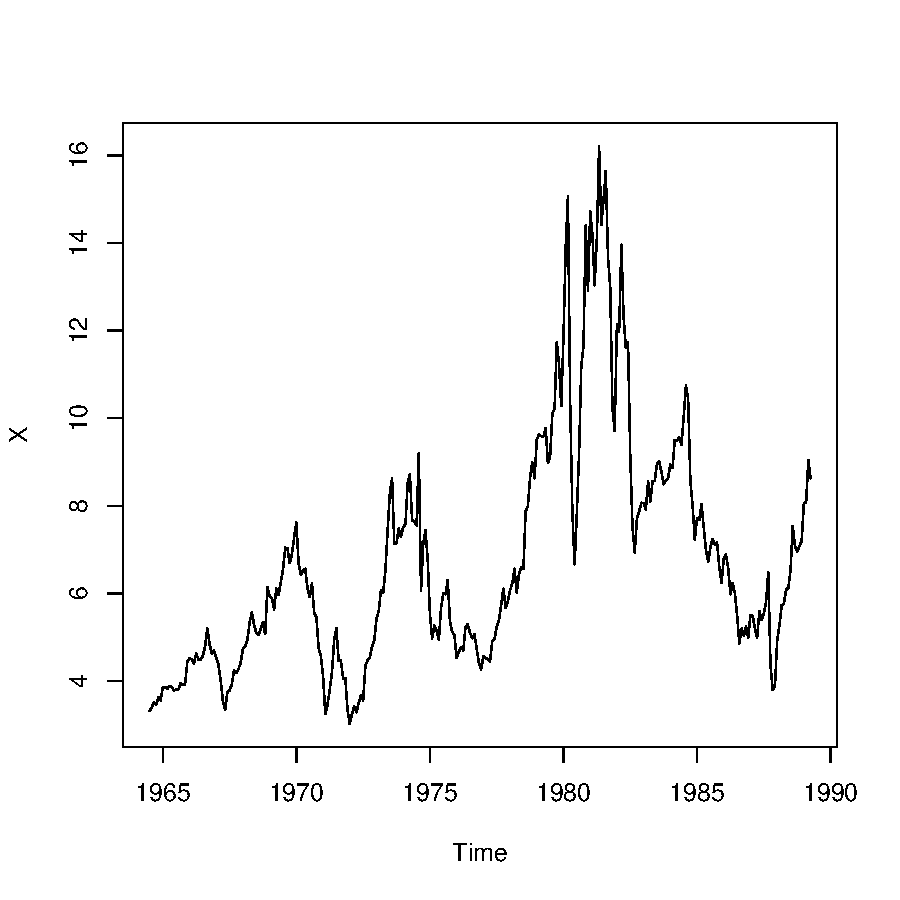
\includegraphics{FitSDE-022}
\end{center}
\caption{The U.S. Interest Rates monthly data from $06/1964$ to $12/1989$.}\label{fig1}
\end{figure}

we can now use all previous methods by \code{fitsde} function to estimate the parameters of model \eqref{eq09} as follows:
\begin{Schunk}
\begin{Sinput}
> fx <- expression( theta[1]+theta[2]*x ) ## drift coefficient of model (9)
> gx <- expression( theta[3]*x^theta[4] ) ## diffusion coefficient of model (9)
> pmle <- eval(formals(fitsde.default)$pmle)
> fitres <- lapply(1:4, function(i) fitsde(X,drift=fx,diffusion=gx,pmle=pmle[i],
+                  start = list(theta1=1,theta2=1,theta3=1,theta4=1)))
> Coef <- data.frame(do.call("cbind",lapply(1:4,function(i) coef(fitres[[i]]))))
> Info <- data.frame(do.call("rbind",lapply(1:4,function(i) logLik(fitres[[i]]))),
+                    do.call("rbind",lapply(1:4,function(i) AIC(fitres[[i]]))),
+                    do.call("rbind",lapply(1:4,function(i) BIC(fitres[[i]]))),
+                    row.names=pmle)
> names(Coef) <- c(pmle)
> names(Info) <- c("logLik","AIC","BIC")
> Coef	
\end{Sinput}
\begin{Soutput}
            euler    kessler      ozaki      shoji
theta1  2.0769516  2.1433505  2.1153154  2.1015009
theta2 -0.2631871 -0.2743368 -0.2690547 -0.2664674
theta3  0.1302158  0.1259800  0.1265225  0.1316708
theta4  1.4513173  1.4691660  1.4649140  1.4513080
\end{Soutput}
\begin{Sinput}
> Info
\end{Sinput}
\begin{Soutput}
           logLik      AIC      BIC
euler   -237.8786 483.7572 487.1514
kessler -237.7845 483.5690 486.9632
ozaki   -237.8356 483.6712 487.0654
shoji   -237.8786 483.7572 487.1514
\end{Soutput}
\end{Schunk}
In Figure \ref{fig2} we reports the sample mean of the solution of the model \eqref{eq20} with the estimated parameters and real data, their empirical $95\%$ confidence bands (from the $2.5th$ to the $97.5th$ percentile), we can proceed as follows:
\begin{equation}\label{eq20}
  dX_{t} = (2.076-0.263 X_{t}) dt + 0.130 X_{t}^{1.451} dW_{t},
\end{equation}
\begin{Schunk}
\begin{Sinput}
> f <- expression( (2.076-0.263*x) )
> g <- expression( 0.130*x^1.451 )
> mod <- snssde1d(drift=f,diffusion=g,x0=X[1],M=200, N=length(X),t0=1964.471,
+                  T=1989.333)
> mod
\end{Sinput}
\begin{Soutput}
Ito Sde 1D:
	| dx = (2.076 - 0.263 * x) * dt + 0.13 * x^1.451 * dw
Method:
	| Euler scheme of order 0.5
Summary:
	| Size of process       | N  = 298.
	| Number of simulation  | M  = 200.
	| Initial value         | x0 = 3.317.
	| Time of process       | t in [1964.471,1989.333].
	| Discretization        | Dt = 0.08342953.
\end{Soutput}
\end{Schunk}
\begin{Schunk}
\begin{Sinput}
> plot(mod,plot.type="single",type="n",ylim=c(0,30))
> lines(X,col=4,lwd=2)
> lines(time(mod),mean(mod),col=2,lwd=2)
> lines(time(mod),bconfint(mod,level=0.95)[,1],col=5,lwd=2)
> lines(time(mod),bconfint(mod,level=0.95)[,2],col=5,lwd=2)
> legend("topleft",c("real data","mean path",paste("bound of", 95,"% confidence")),
+        inset = .01,col=c(4,2,5),lwd=2,cex=0.8)
\end{Sinput}
\end{Schunk}
\setkeys{Gin}{width=0.5\textwidth}
\begin{figure}[!ht]
\begin{center}
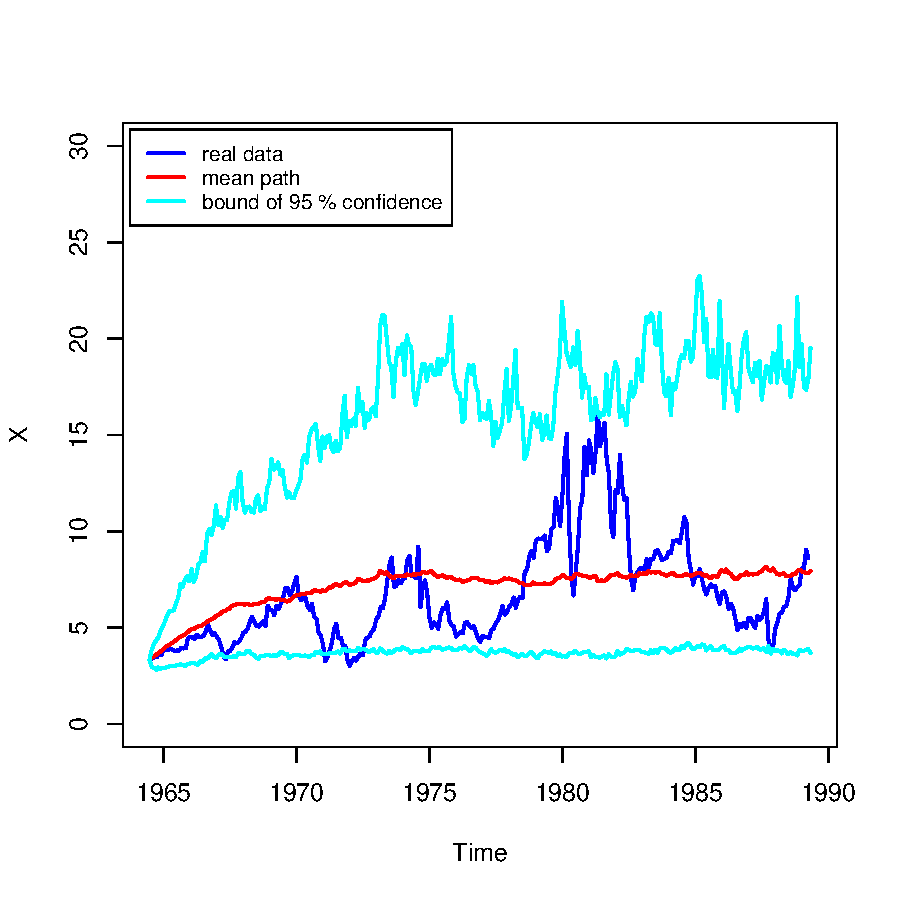
\includegraphics{FitSDE-026}
\end{center}
\caption{Real data vs the empirical mean of $200$ simulated trajectories of model \eqref{eq20}.}\label{fig2}
\end{figure}

\section{Summary}
The asymptotic approach to statistical estimation is frequently adopted because of its general applicability and relative simplicity. In this work we explained the use of \code{fitsde} function in \pkg{Sim.DiffProc} package, which is based on pseudo-maximum likelihood estimator for one-dimensional stochastic differential equations, with different approximation methods and some examples of applications.

\begin{thebibliography}{1}
\expandafter\ifx\csname natexlab\endcsname\relax\def\natexlab#1{#1}\fi
\expandafter\ifx\csname url\endcsname\relax
  \def\url#1{{\tt #1}}\fi

\bibitem[Dacunha and Florens, 1986]{DacunhaandFlorens1986}
Dacunha, D.C. and Florens, D.Z. (1986).
\newblock Estimation of the Coefficients of a Diffusion from Discrete Observations.
\newblock \emph{Stochastics}. 19, 263--284.

\bibitem[Florens, 1989]{Florens1989}
Florens, Z.D. (1989).
\newblock Approximate discrete time schemes for statistics of diffusion processes.
\newblock \emph{Statistics}. 20, 547--557.

\bibitem[Dohnal, 1987]{Dohnal1987}
Dohnal, G. (1987).
\newblock On estimating the diffusion coefficient.
\newblock \emph{J. Appl.Prob.}, 24, 105--114.

\bibitem[Genon, 1990]{Genon1990}
Genon, V.C. (1990).
\newblock Maximum constrast estimation for diffusion processes from discrete observation.
\newblock \emph{Statistics}, 21, 99--116.

\bibitem[A\"{\i}t-Sahalia, 1999]{AitSahalia1999}
A\"{\i}t-Sahalia, Y. (1999).
\newblock Transition densities for interest rate and other nonlinear diffusions.
\newblock \emph{The Journal of Finance}, 54, 1361--1395.

\bibitem[A\"{\i}t-Sahalia, 2002]{AitSahalia2002}
A\"{\i}t-Sahalia, Y. (2002).
\newblock Maximum likelihood estimation of discretely sampled diffusions: a closed-form approximation approach.
\newblock \emph{Econometrica}. 70, 223--262.

\bibitem[Kessler, 1997]{Kessler1997}
Kessler, M. (1997).
\newblock Estimation of an ergodic diffusion from discrete observations.
\newblock \emph{Scand. J. Statist.}, 24, 211-229.

\bibitem[Ozaki, 1992]{Ozaki1992}
Ozaki, T. (1992).
\newblock A bridge between nonlinear time series models and nonlinear stochastic dynamical systems: A local linearization approach.
\newblock \emph{Statistica Sinica}, 2, 25-83.

\bibitem[Shoji and Ozaki, 1997]{ShojiandOzaki1997}
Shoji, L. and Ozaki, T. (1997).
\newblock Comparative study of estimation methods for continuous time stochastic processes.
\newblock \emph{J.Time Ser. Anal.,} 18, 485--506.

\bibitem[Shoji and Ozaki, 1998]{ShojiandOzaki1998}
Shoji, L. and Ozaki, T. (1998).
\newblock  Estimation for nonlinear stochastic differential equations by a local linearization method.
\newblock  \emph{Stochastic Analysis and Applications}, 16, 733-752.

\bibitem[Nicolau, 2002]{Nicolau2002}
Nicolau, J. (2002).
\newblock New Technique for Simulating the Likelihood of Stochastic Differential Equations.
\newblock \emph{The Econometrics Journal}. 5(1).

\bibitem[Nicolau, 2004]{Nicolau2004}
Nicolau, J. (2004).
\newblock  Introduction to the estimation of stochastic differential equations based on discrete observations.
\newblock  \emph{Autumn School and International Conference, Stochastic Finance}.

\bibitem[Boukhetala, 1996]{Boukhetala1996}
Boukhetala, K. (1996).
\newblock Modelling and simulation of a dispersion pollutant with attractive centre.
\newblock ed by Computational Mechanics Publications, Southampton ,U.K and Computational Mechanics Inc, Boston, USA, 245--252.

\bibitem[Stefano, 2008]{Stefano2008}
Stefano, M.I. (2008).
\newblock \emph{Simulation and inference for stochastic differential equations: with \R~examples}.
\newblock Springer-Verlag, New York.

\bibitem[Stefano, 2009]{Stefano2009}
Stefano, M.I. (2009).
\newblock \CRANpkg{sde}: Simulation and Inference for Stochastic Differential Equations.
\newblock \emph{\R~package version 2.0.10}.
\newblock \url{http://CRAN.R-project.org/package=sde}

\bibitem[Stefano, 2011]{Stefano2011}
Stefano, M.I. (2011).
\newblock \emph{Option Pricing and Estimation of Financial Models with \R}.
\newblock John Wiley \& Sons Ltd.

\bibitem[Stefano et all, 2014]{Stefano2014}
Alexandre Brouste, Masaaki Fukasawa, Hideitsu Hino, Stefano M. Iacus, Kengo Kamatani, Yuta Koike, Hiroki Masuda, Ryosuke Nomura, Teppei Ogihara, Yasutaka Shimuzu, Masayuki Uchida, Nakahiro Yoshida. (2014).
\newblock The \CRANpkg{yuima} Project: A Computational Framework for Simulation and Inference of Stochastic Differential Equations.
\newblock \emph{Journal of Statistical Software}, 57(4). 1--51.
\newblock \url{http://www.jstatsoft.org/v57/i04/}.

\bibitem[Brouste and Stefano, 2013]{BrousteandStefano2013}
Brouste, A. and Stefano, M.I. (2013).
\newblock Parameter Estimation for the Discretely Observed Fractional Ornstein-Uhlenbeck Process and the \pkg{yuima} \R~Package.
\newblock \emph{Computational Statistics}. 28(4), 1129--1147.

\bibitem[Guidoum and Boukhetala, 2014]{Sim.DiffProc}
Guidoum, A. C. and Boukhetala, K. (2014).
\newblock \CRANpkg{Sim.DiffProc}: Simulation of Diffusion Processes.
\newblock \R~package version 2.7.
\newblock \url{http://CRAN.R-project.org/package=Sim.DiffProc}

\bibitem[Guidoum and Boukhetala, 2014b]{}
Guidoum, A. C. and Boukhetala, K. (2014).
\newblock Quasi Maximum Likelihood Estimation for One-Dimensional Diffusion Processes.
\newblock In submission (The \R~Journal).

\bibitem[\R~Development Core Team (2014)]{R}
\R~Development Core Team (2014).
\newblock {\em \R: A Language and Environment for Statistical Computing}.
\newblock Vienna, Austria.
\newblock \url{http://www.R-project.org/}

\bibitem[Stig and S{\o}ren, 2013]{StigandSoren2013}
Stig, M. and S{\o}ren, K. (2013).
\newblock \CRANpkg{PSM}: Non-Linear Mixed-Effects modelling using Stochastic Differential Equations.
\newblock \emph{\R~package version 0.8-10}.
\newblock \url{http://CRAN.R-project.org/package=PSM}

\bibitem[Croissant, 2014]{Croissant2014}
Croissant, Y. (2014).
\newblock \CRANpkg{Ecdat}: Data Sets for Econometrics.
\newblock \emph{\R~package version 0.2-4}.
\newblock \url{http://CRAN.R-project.org/package=Ecdat}

\bibitem[Prakasa, 1999]{Prakasa1999}
B.L.S. Prakasa Rao. (1999).
\newblock \emph{Statistical Inference for Diffusion Type Processes}.
\newblock Arnold, London and Oxford University press, New York.

\bibitem[Florens, 1999]{Florens1999}
Florens, D. (1999).
\newblock Estimation of the diffusion coefficient from the crossings,
\newblock \emph{Stat. Infer. Stochastic Process}. 1, 175--195.

\bibitem[Kutoyants, 2004]{Kutoyants2004}
Kutoyants, Y.A. (2004).
\newblock S\emph{tatistical Inference for Ergodic Diffusion Processes}.
\newblock Springer, London.

\bibitem[S{\o}rensen, 2000]{Sorensen2000}
S{\o}rensen, H. (2000).
\newblock Inference for Diffusion Processes and Stochastic Volatility Models.
\newblock Ph.D. thesis, Department of Mathematical Sciences, University of Copenhagen.

\bibitem[S{\o}rensen, 2002]{Sorensen2002}
S{\o}rensen, H. (2002).
\newblock Estimation of diffusion parameters for discretely observed diffusion processes.
\newblock \emph{Bernoulli}, 8, 491--508.

\bibitem[S{\o}rensen, 2004]{Sorensen2004}
S{\o}rensen, H. (2004).
\newblock Parametric inference for diffusion processes observed at discrete points in time: a survey.
\newblock \emph{International Statistical Review}, 72, 337--354.

\bibitem[Hurn and Lindsay, 1999]{HurnandLindsay1999}
Hurn, A.S. and Lindsay, K.A. (1999).
\newblock Estimating the parameters of stochastic differential equations.
\newblock \emph{Mathematics And Computers In Simulation}. 48, 373--384.

\bibitem[Hurn et all, 2003]{Hurnetall2003}
Hurn, A.S., Lindsay, K.A. and Martin, V.L. (2003).
\newblock On the efficacy of simulated maximum likelihood for estimating the parameters of stochastic differential equations.
\newblock \emph{Journal of Time Series Analysis}. 24(1), 45--63.

\bibitem[Pedersen, 1995]{Pedersen1995}
Pedersen, A.R. (1995).
\newblock A new approach to maximum likelihood estimation for stochastic differential equations based on discrete observations.
\newblock \emph{Scand. J. Statist.}, 22(1), 55--71.

\bibitem[Yoshida, 1992]{Yoshida1992}
Yoshida, N. (1992).
\newblock Estimation of diffusion processes from discrete observations.
\newblock \emph{Journal of Multivariate Analysis}. 41, 220--242.

\bibitem[Gallant and Long, 1997]{GallantandLong1997}
Gallant, A and Long, J. (1997).
\newblock Estimating stochastic differential equations efficiently by minimum chi-square.
\newblock \emph{Biometrika}. 84, 124--141.

\bibitem[Alcock and Burrage, 2004]{AlcockandBurrage2004}
Alcock, J and Burrage, K. (2004).
\newblock A genetic estimation algorithm for parameters of stochastic ordinary differential equations.
\newblock \emph{Computational Statistics \& Data Analysis}. 47, 255--275.

\bibitem[Ogihara and Yoshida, 2011]{OgiharaandYoshida2011}
Ogihara, T. and Yoshida, N. (2011).
\newblock  Quasi-Likelihood Analysis for the Stochastic Differential Equation with Jumps.
\newblock \emph{Statistical Inference for Stochastic Processes}. 14(3), 189--229.

\bibitem[Uchida and Yoshida, 2005]{UchidaandYoshida2005}
Uchida, M. and Yoshida, N. (2005).
\newblock AIC for ergodic diffusion processes from discrete observations.
\newblock \emph{preprint MHF 2005-12, March 2005, Faculty of Mathematics, Kyushu University}. Fukuoka, Japan.

\bibitem[Uchida and Yoshida, 2012]{UchidaandYoshida2012}
Uchida, M. and Yoshida, N. (2012).
\newblock Adaptive Estimation of an Ergodic Diffusion Process Based on Sampled Data.
\newblock \emph{Stochastic Processes and their Applications}. 122(8), 2885--2924.

\bibitem[Kloeden et all, 1996]{Kloedenetall1996}
Kloeden, P., Platen, E., Schurz and S{\o}rensen, M. (1996).
\newblock On Effects of Discretization on Estimators of Drift Parameters for Diffusion Processes.
\newblock \emph{Journal of Applied Probability}. 33, 1061--1076.

\end{thebibliography}


